\chapter{Implementation}

%Explain what you did to implement your solution, problems that occurred and how you fixed them. 
%If they are interesting, include some relevant parts of the implementation (most relevant pieces of code and so on). 

\section{Communication Protocols}


Centralized pool, robots, charging stations and sensors need to share information with each other.
To improve the communication efficiency, communication protocols are designed. 

\subsection{Message about Measurement}
\label{sec:measurement_message}
When a robot passes by a door, it should receive messages from a sensor. In this project, we use a ROS node "sensor simulator" to simulate door sensors (Section \ref{sec:sensor_simulatior}) to publish instant measurement result (Table \ref{tab:sensor_message}).

\begin{table}[htb]
\centering
\begin{tabular}{|c|c|c|c|c|} 
\hline
Door ID  & Position& Timestamp & Measurement Result \\
\hline\hline
1&(-18.5,5.2) & 2020-06-01 9:00:02 & Door opened \\ [1ex] 
\hline
\end{tabular}
\caption{Measurement Message Format and Example}
\label{tab:sensor_message}
\end{table}
	

\subsection{Message about Task}
\label{sec:task_message}
There are some basic requirements for communication between robot and centralized pool: firstly,
robot should initiate the communication once it has finished all task in task queue and get free. 
Secondly, robot should forward sensor data to centralized pool while processing a task. 
These Communication protocols save unnecessary communication cost by avoiding keep tracking the current position, availability and states of all robots (Figure \ref{fig:comminication}).
Four types of message are defined: 
(1)Task request message(Table\ref{tab:request_message}); (2) Task goal messages(Table \ref{tab:goal_message}); (3) Task feedback message (Table \ref{tab:feedback_message}); (4) Task result message (Table \ref{tab:result_message}). 

\begin{figure}[htbp]
    \centering
    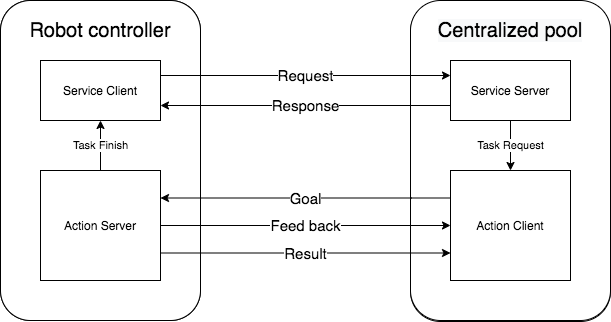
\includegraphics[width = 0.7\textwidth]{content/images/ch4/robot_pool_comminication.drawio.png}
    \caption{Communication between Robot and Centralized Pool}
    \label{fig:comminication}
\end{figure}

\begin{table}[htb]
\centering
\begin{tabular}{|c|c|c|} 
\hline
Battery Level & Position & Robot ID\\
\hline\hline
93	&(2,4)	&1 \\ [1ex] 
\hline
\end{tabular}
\caption{Request Message Format and Example}
\label{tab:request_message}
\end{table}

\begin{table}[htb]
\centering
\resizebox{\textwidth}{!}{
\begin{tabular}{|c|c|c|c|} 
\hline
Task ID-[] &Task type & Target ID & Goal[] \\
\hline\hline
1& Gather Environment Info & 9	& (-1.5,5.2) 2020-06-01 9:00:00 \\
\hline
[3,4]	& Execute task & 21, 22	& (-24.0,12.0), 2020-06-01 9:02:00 (-21.0,12.0) 2020-06-01 9:02:00 \\
\hline
5	& Charging	& 17	&(0.0,5.0), 2020-06-01 9:04:00 \\ [1ex] 
\hline
\end{tabular}}
\caption{Action Goal Message Format and Example}
\label{tab:goal_message}
\end{table}

\begin{table}[htb]
\centering
\begin{tabular}{|c|c|c|c|} 
\hline
Robot ID & Door ID & Measurement time & Measurement result \\
\hline\hline
1	& 3	& 2020-06-01 9:00:03 & Door open \\ [1ex] 
\hline
\end{tabular}
\caption{Action Feedback Message Format and Example}
\label{tab:feedback_message}
\end{table}

\begin{table}[htb]
\centering
\begin{tabular}{|c|c|c|} 
\hline
Task ID 	& Task type	& Result\\
\hline\hline
1 & Gather Environment Info & Success \\ [1ex] 
\hline
\end{tabular}
\caption{Action Result Message Format and Example}
\label{tab:result_message}
\end{table}


\begin{table}[htb]
\centering
\begin{tabular}{|c|c|c|} 
\hline
Robot ID & Battery Level \\
\hline\hline
1 & 93 \\ [1ex] 
\hline
\end{tabular}
\caption{Message to Charging Station}
\label{tab:message_to_charging_staion}
\end{table}

\subsection{Message about Charging}
  
When a robot arrives charging station's position, it sends a message to Charging station(Figure \ref{tab:message_to_charging_staion}). The details of charging station is discussed in Section \ref{sec:charging_station}. 

\section{Database}
The centralized pool keep environment information in database to make decisions. The structure of database is shown in Figure \ref{fig:database_er}. Following are explanations of some tables.
\begin{itemize}
    \item \textsl{Table measurements} Table ``measurements'' (Figure \ref{tab:db_measurement_result}) stores measurement result.
    \item \textsl{Table doors.} Table ``doors'' stores environment information. In table ``doors'', the ``is used'' column will be updated when the centralized pool gives a robot a task to the corresponding door. The ``last update'' column will be updated when the centralized pool receives a new measurement result of the corresponding door. 
	\item \textsl{Table open\_ossibilities.} Table ``open possibilities'' (Figure \ref{tab:db_open_possibilities}) is based on the statistic of measurement result in ``measurement'' table in a specific time period of each working day. These two table will be updated when centralized pool receive a new measurement result. 
	\item \textsl{Table exe\_rs.} Table ``exe rs'' stores experiment result while table ``exe weight'', table ``door weight'' and table ``charging station weight'' store weight values for experiment. Chapter 5 introduces the details of experiment.
	\item \textsl{Table costum\_points.} When a task is created, the target point of this task will be stored in ``position'' table, and a ``target ID'' will be generated.  This ``target ID'' will be stored in ``custom points'' table. Additionally, with the information in ``room range'' table, the system will recognize which room does the point belong to and write ``room ID'' column in ``custom points'' table.
\end{itemize}

\begin{table}[htb]
    \centering
    \begin{tabular}{|c|c|c|} 
    \hline
    Table Name & Column Name & Explanation \\
    \hline
    \multirow{3}*{Measurements} &  door ID & door ID\\
    \cline{2-3}  
    ~ &  door status & measurement "door opened" or "door close" \\
    \cline{2-3}
    ~ &  date time & measurement timestamp\\
    \hline
    \end{tabular}
    \caption{}
    \label{tab:}
    \end{table}
\begin{figure}[htbp]
    \centering
    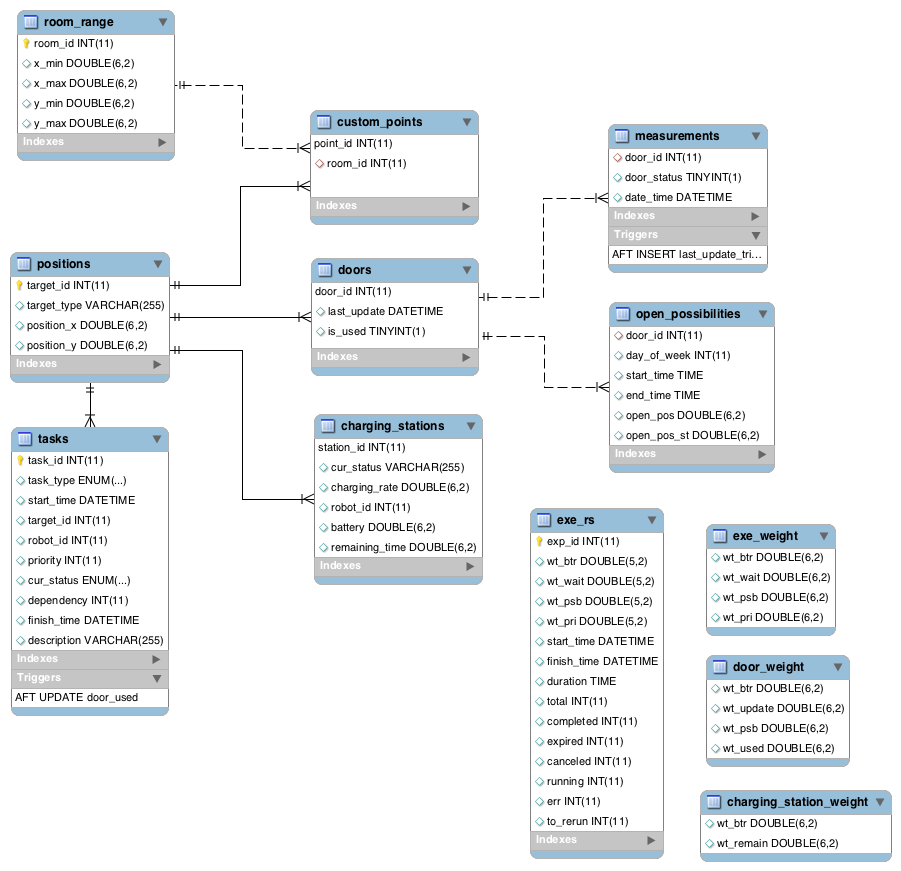
\includegraphics[width = 0.8\textwidth]{content/images/ch4/database_er.png}
    \caption{Database Entity Relationship Diagram}
    \label{fig:database_er}
\end{figure}


\begin{table}[htb]
\centering
\begin{tabular}{|c| c| c|} 
\hline
Door ID & Door Status & Date Time \\
\hline
1& 1 & 2020-06-01 09:00:01 \\ [1ex] 
\hline
\end{tabular}
\caption{Measurement Result}
\label{tab:db_measurement_result}
\end{table}

\begin{table}[htb]
\centering
\resizebox{\textwidth}{!}{
\begin{tabular}{|c|c| c| c| c| c|} 
\hline
Door id & Day Of Week & Start Time & End Time & Initialized Open Possibility &  Open Possibility Statistic \\
\hline
1 & 2 & 10:00:00 & 10:59:59 & 0.80 & 0.80 \\ [1ex] 
\hline
1 & 2 & 11:00:00 & 11:59:59 & 0.20 & 0.18 \\ [1ex] 
\hline
2 & 2 & 10:00:00 & 10:59:59 & 0.80 & 0.82 \\ [1ex] 
\hline
\end{tabular}}
\caption{Door Open Possibility}
\label{tab:db_open_possibilities}
\end{table}


\section{Procedure}
As stated in the Chapter 3, the goal of task scheduling is finishing all tasks as soon as possible while keep the cost as low as possible. 
The task assignment and execution has at two level. \cite{Ivan2017} the task and the path planner solves a planning problem. It takes and occupancy grid, a specific robot and a set of task specifications, and generates trajectories for each task. According to those trajectories and task specifications, the task with the lowest cost is assigned to robot.
At the dynamic level, after each robot receive a task, it runs a navigation stack to execute this task stepwise. Each robot computes a local trajectory but takes into account dynamic obstacles.
The process of the robot task allocation system is as follows.

\begin{figure}[htbp]
    \centering
    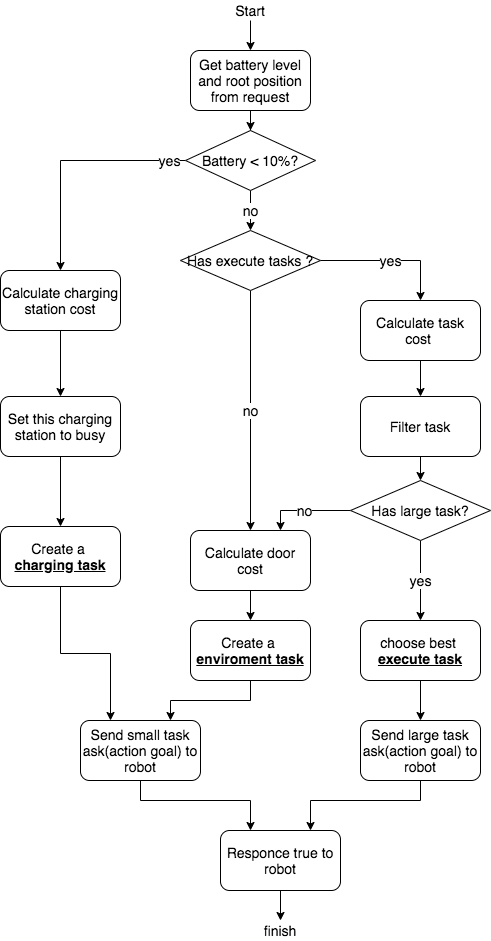
\includegraphics[width = 0.7\textwidth]{content/images/ch4/centralized_task_select.drawio.png}
    \caption{Centralized Pool Task Allocation}
    \label{fig:centralized_task_allocation}
\end{figure}
\subsection{Centralized Pool}

\paragraph{Task Allocation}
The task allocation algorithm is discussed in Section \ref{sec:exe_task_allocation}. The process of task allocation is shown in Figure \ref{fig:centralized_task_allocation}. 

\paragraph{Handle Task Feedback.}
When the centralized pool receives a task feedback (Table \ref{tab:feedback_message}) that contains a new measurement result from robot, it will add a record in measurement table and update ``open possibilities'' table in database.

\paragraph{Handle Task Result.}
When the centralized pool receives a task result (Table \ref{tab:result_message}), it updates ``tasks'' table. The failed ``execute tasks'' will be reused whileothers will be marked as ``Cancel'' or ``Error''(Figure \ref{fig:centralized_task_handle}).

\begin{figure}[htbp]
    \centering
    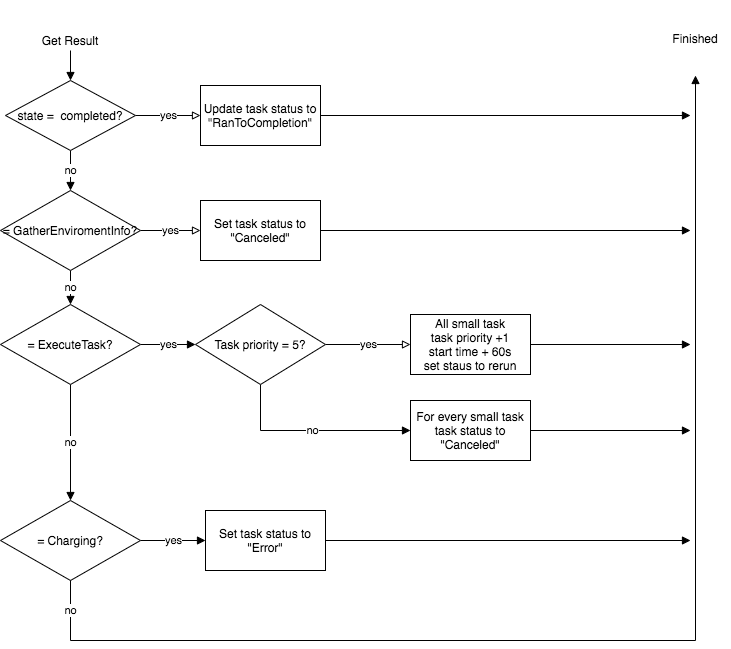
\includegraphics[width = 0.7\textwidth]{content/images/ch4/centralized_task_result.drawio.png}
    \caption{Centralized Pool Handle Task Result}
    \label{fig:centralized_task_handle}
\end{figure}


\subsection{Robot}

\begin{figure}[htbp]
    \centering
    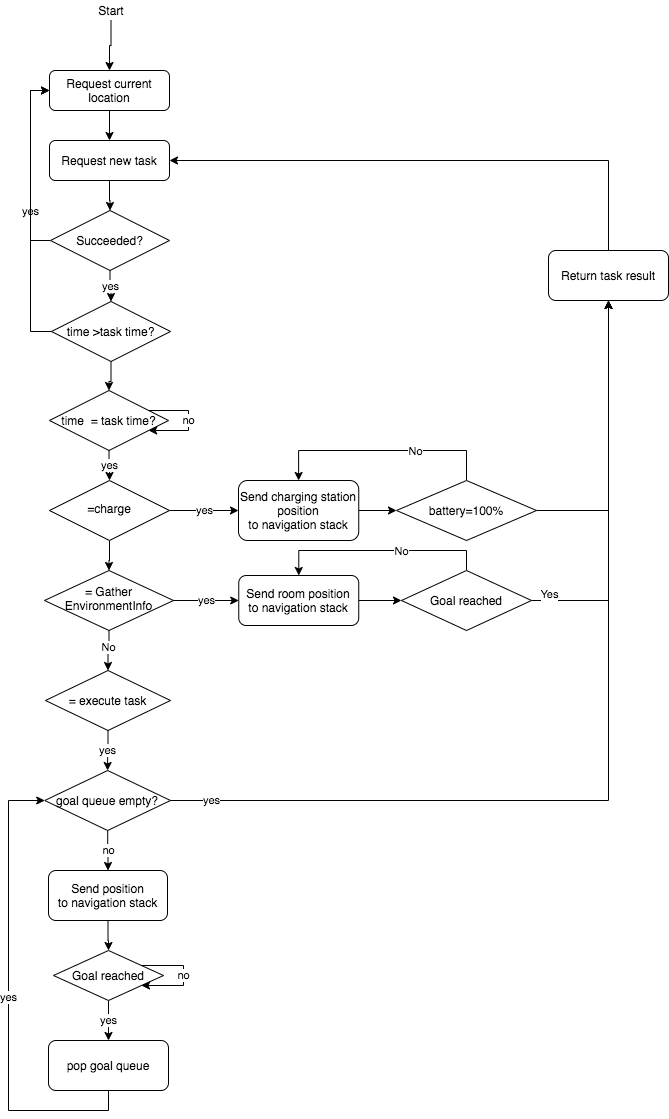
\includegraphics[width = 0.7\textwidth]{content/images/ch4/robot_process_task.drawio.png}
    \caption{Robot Process Task }
    \label{fig:task_process_robot}
\end{figure}

\paragraph{Robot Process Tasks}
When the task queue(Figure \ref{fig:system_architecture}) in a robot is empty, the robot requests a new task. If the robot gets a ``charging task'', it will move to the position of charging staion(Figure \ref{fig:positions_door_station}) and interact with charging station node (Section \ref{sec:charging_station}).
When a robot gets an ``execute task'' which is a large task, it will move to all goals in order.
When a robot gets a ``gather environment information'' task, it will move to the door's position.
During task processing, the timer checks periodically the status of navigation stack. If any errors occurs, the robot send a ``failed'' result with description to the centralized pool.  
When all tasks are complted without error, the robot will send ``Succedded'' result to the centralized pool.


\begin{figure}[htbp]
    \centering
    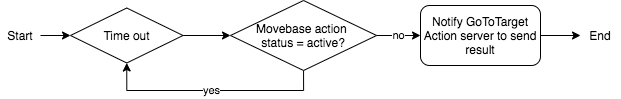
\includegraphics[width = 0.7\textwidth]{content/images/ch4/robot_timer.drawio.png}
    \caption{Robot Timer}
    \label{fig:robot_timer}
\end{figure}

\begin{figure}[htbp]
    \centering
    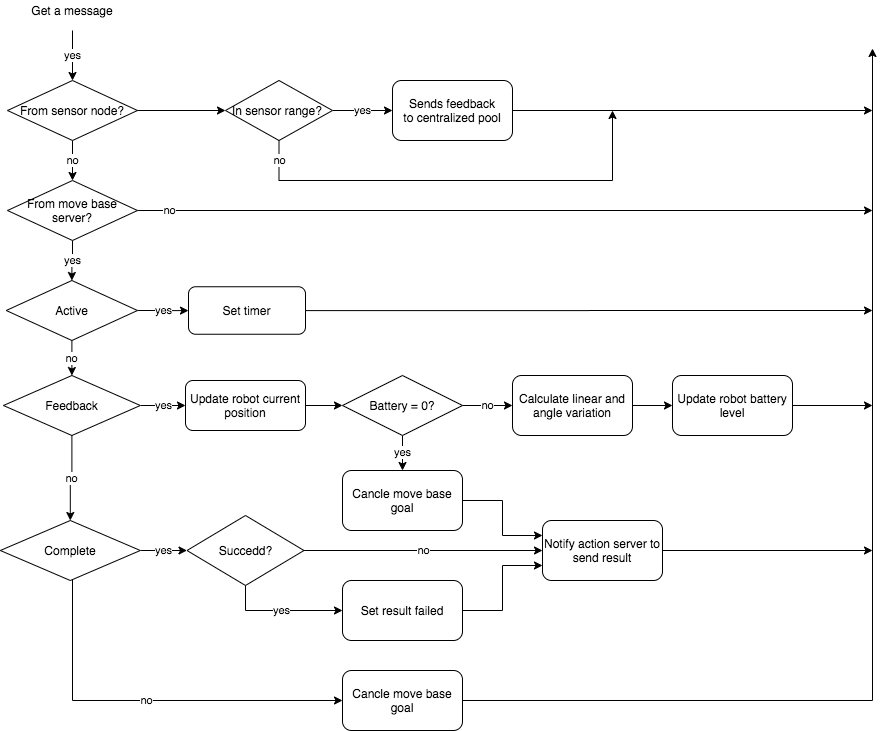
\includegraphics[width = 0.7\textwidth]{content/images/ch4/robot_message.drawio.png}
    \caption{Robot Handle Message}
    \label{fig:robot_handle_message}
\end{figure}

\paragraph{Robot Handle Messages}
While a robot is processing a task, it listens to door sensors and forwards measurement result to the centralized pool. 
Besides messages from sensor, it also receives messages from ``move\_base'' node. The details of robot message handling is shown in Figure \ref{fig:robot_handle_message}.

\subsection{Charging Station}
\label{sec:charging_station}
The charging station consists of a charging station node and ``charging station'' table in database (Table \ref{fig:database_er}). 
When a robot arrives the position of charging station, it will start interacting with charging station node. Once the charging station receives robot information(Figure \ref{fig:charging_station_message}), its state will be changed to ``charging''(Figure \ref{fig:charging_station_state_machine}) and its ``battery level'' will be increased and its ``remaining time'' will be decreased(Figure \ref{fig:charging_station_event}).  
Once finishing charging, its status will be set ``charging finish''. When robot leaves charging station, its status will be set to ``free''. 


\begin{figure}[htbp]
    \centering
    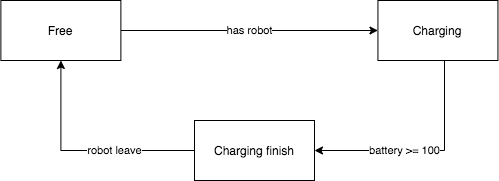
\includegraphics[width = 0.7\textwidth]{content/images/ch4/charging_station_state_machine.drawio.png}
    \caption{Charging Station State Machine}
    \label{fig:charging_station_state_machine}
\end{figure}

\begin{figure}[htbp]
    \centering
    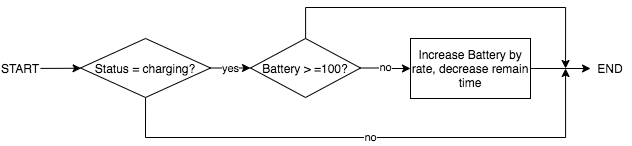
\includegraphics[width = 0.7\textwidth]{content/images/ch4/charging_station_charging_event.drawio.png}
    \caption{Charging Station Scheduled Charging Event}
    \label{fig:charging_station_event}
\end{figure}

\begin{figure}[htbp]
    \centering
    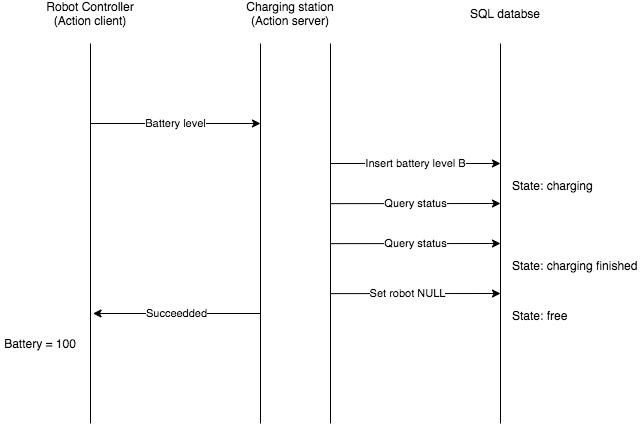
\includegraphics[width = 0.9\textwidth]{content/images/ch4/charging_station_message.drawio.png}
    \caption{Charging Station Message}
    \label{fig:charging_station_message}
\end{figure}

\subsection{Sensor Simulator}



\label{sec:sensor_simulatior}
The simulator \todo{sensor simulator}

\begin{figure}[htbp]
    \centering
    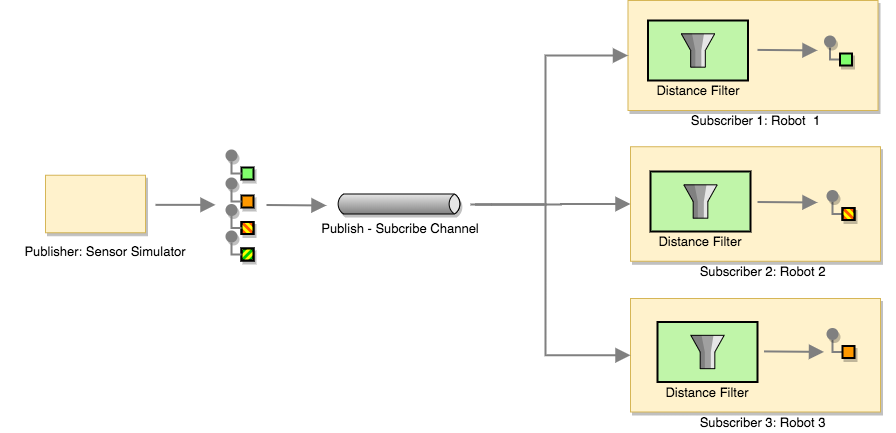
\includegraphics[width = 0.7\textwidth]{content/images/ch4/sensor_simulator.drawio.png}
    \caption{Sensor Simulator}
    \label{}
\end{figure}